% Options for packages loaded elsewhere
\PassOptionsToPackage{unicode}{hyperref}
\PassOptionsToPackage{hyphens}{url}
%
\documentclass[
]{article}
\usepackage{lmodern}
\usepackage{amssymb,amsmath}
\usepackage{ifxetex,ifluatex}
\ifnum 0\ifxetex 1\fi\ifluatex 1\fi=0 % if pdftex
  \usepackage[T1]{fontenc}
  \usepackage[utf8]{inputenc}
  \usepackage{textcomp} % provide euro and other symbols
\else % if luatex or xetex
  \usepackage{unicode-math}
  \defaultfontfeatures{Scale=MatchLowercase}
  \defaultfontfeatures[\rmfamily]{Ligatures=TeX,Scale=1}
\fi
% Use upquote if available, for straight quotes in verbatim environments
\IfFileExists{upquote.sty}{\usepackage{upquote}}{}
\IfFileExists{microtype.sty}{% use microtype if available
  \usepackage[]{microtype}
  \UseMicrotypeSet[protrusion]{basicmath} % disable protrusion for tt fonts
}{}
\makeatletter
\@ifundefined{KOMAClassName}{% if non-KOMA class
  \IfFileExists{parskip.sty}{%
    \usepackage{parskip}
  }{% else
    \setlength{\parindent}{0pt}
    \setlength{\parskip}{6pt plus 2pt minus 1pt}}
}{% if KOMA class
  \KOMAoptions{parskip=half}}
\makeatother
\usepackage{xcolor}
\IfFileExists{xurl.sty}{\usepackage{xurl}}{} % add URL line breaks if available
\IfFileExists{bookmark.sty}{\usepackage{bookmark}}{\usepackage{hyperref}}
\hypersetup{
  pdftitle={linear norm plot},
  pdfauthor={Joshua},
  hidelinks,
  pdfcreator={LaTeX via pandoc}}
\urlstyle{same} % disable monospaced font for URLs
\usepackage[margin=1in]{geometry}
\usepackage{graphicx,grffile}
\makeatletter
\def\maxwidth{\ifdim\Gin@nat@width>\linewidth\linewidth\else\Gin@nat@width\fi}
\def\maxheight{\ifdim\Gin@nat@height>\textheight\textheight\else\Gin@nat@height\fi}
\makeatother
% Scale images if necessary, so that they will not overflow the page
% margins by default, and it is still possible to overwrite the defaults
% using explicit options in \includegraphics[width, height, ...]{}
\setkeys{Gin}{width=\maxwidth,height=\maxheight,keepaspectratio}
% Set default figure placement to htbp
\makeatletter
\def\fps@figure{htbp}
\makeatother
\setlength{\emergencystretch}{3em} % prevent overfull lines
\providecommand{\tightlist}{%
  \setlength{\itemsep}{0pt}\setlength{\parskip}{0pt}}
\setcounter{secnumdepth}{-\maxdimen} % remove section numbering
\usepackage{booktabs}
\usepackage{longtable}
\usepackage{array}
\usepackage{multirow}
\usepackage{wrapfig}
\usepackage{float}
\usepackage{colortbl}
\usepackage{pdflscape}
\usepackage{tabu}
\usepackage{threeparttable}
\usepackage{threeparttablex}
\usepackage[normalem]{ulem}
\usepackage{makecell}
\usepackage{xcolor}

\title{linear norm plot}
\author{Joshua}
\date{15/05/2020}

\begin{document}
\maketitle

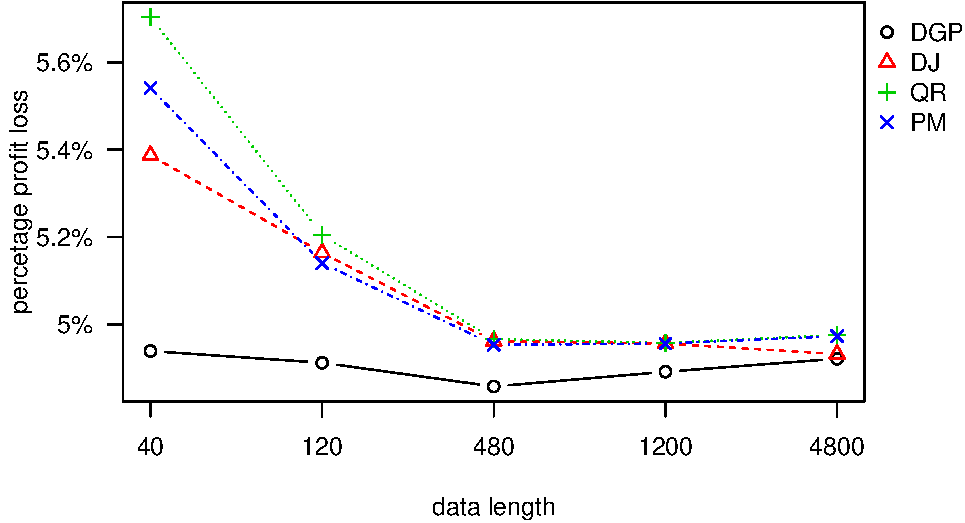
\includegraphics{linear-norm-plot_files/figure-latex/ppl0.5-1.pdf}

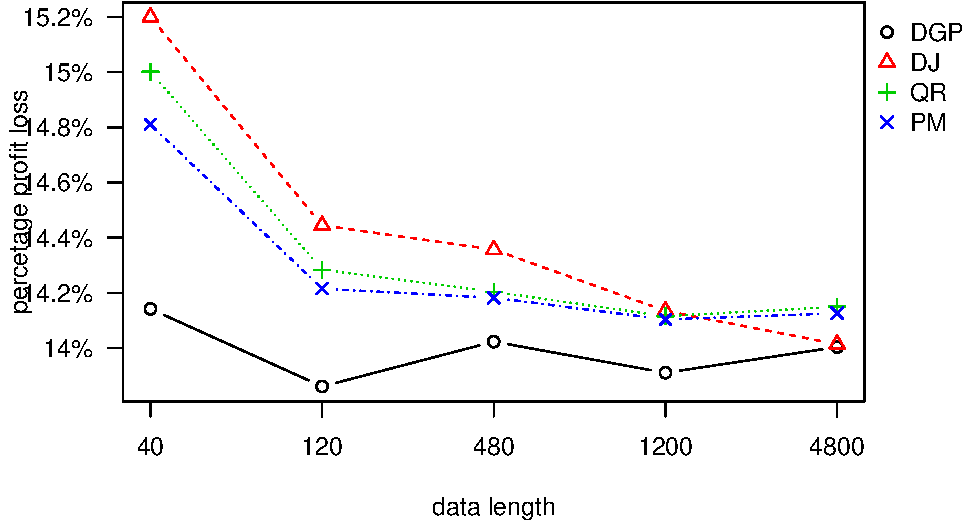
\includegraphics{linear-norm-plot_files/figure-latex/ppl0.63-1.pdf}

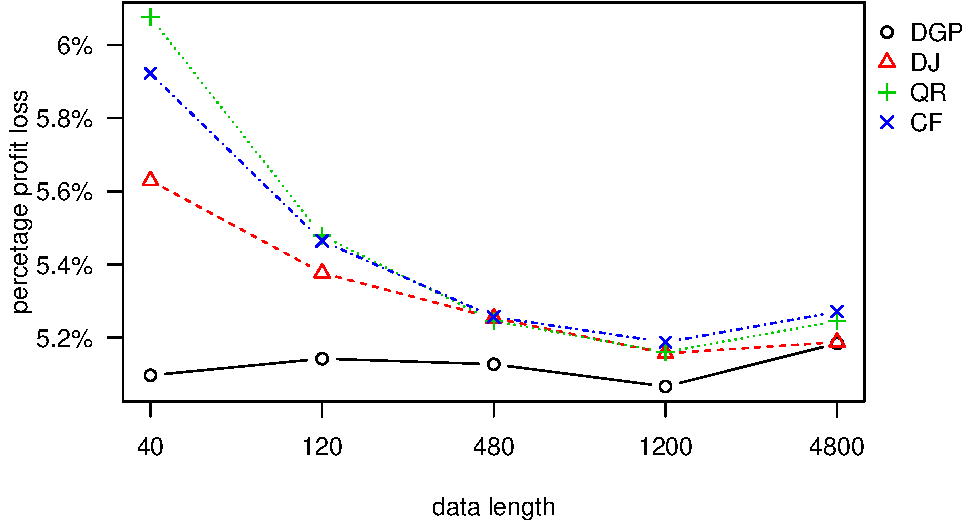
\includegraphics{linear-norm-plot_files/figure-latex/ppl0.3-1.pdf}

\begin{table}

\caption{\label{tab:inventory_error}Inventory Error}
\centering
\resizebox{\linewidth}{!}{
\begin{tabular}[t]{ccccccccccccc}
\toprule
\multicolumn{1}{c}{\textbf{ }} & \multicolumn{4}{c}{\textbf{Target service level=0.5}} & \multicolumn{4}{c}{\textbf{Target service level=0.63}} & \multicolumn{4}{c}{\textbf{Target service level=0.3}} \\
\cmidrule(l{3pt}r{3pt}){2-5} \cmidrule(l{3pt}r{3pt}){6-9} \cmidrule(l{3pt}r{3pt}){10-13}
Data size & DGP & disjoint & quantile & proposed & DGP & disjoint & quantile & proposed & DGP & disjoint & quantile & proposed\\
\midrule
\rowcolor{gray!6}  40 & 0.38 & 30.38 & 0.34 & 0.46 & -65.82 & -17.8 & -28.48 & -28.99 & 103.25 & 105.54 & 53.34 & 48.81\\
 & (100.28) & (114.25) & (116.91) & (112.95) & (100.44) & (114.24) & (117.59) & (113.16) & (100.01) & (114.73) & (117.32) & (112.49)\\
\rowcolor{gray!6}  120 & -0.95 & 8.48 & -1.04 & -1.09 & -45.61 & -31.08 & -33.68 & -32.57 & 70.72 & 73.58 & 52.57 & 50.89\\
 & (100.87) & (111.91) & (106.27) & (105.35) & (100.29) & (112.8) & (106.45) & (105.07) & (99.24) & (110.93) & (104.96) & (103.62)\\
\rowcolor{gray!6}  480 & 0.19 & 3 & 0.22 & 0.23 & -37.19 & -35.73 & -34.12 & -33.84 & 56.99 & 60.59 & 52.51 & 51.94\\
\addlinespace
 & (99.55) & (108.38) & (101.71) & (101.42) & (99.37) & (108.15) & (101.56) & (101.33) & (100.21) & (109.01) & (102.56) & (102.33)\\
\rowcolor{gray!6}  1200 & 1 & 2.22 & 0.96 & 0.98 & -36.64 & -34.92 & -35.77 & -35.52 & 53.58 & 54.35 & 52.03 & 51.67\\
 & (100.58) & (101.45) & (102.15) & (102.09) & (99.69) & (100.72) & (101.12) & (101.01) & (99.67) & (100.79) & (101.21) & (101.21)\\
\rowcolor{gray!6}  4800 & -1.11 & -0.7 & -1.17 & -1.18 & -35.2 & -34.81 & -35.27 & -35.08 & 51.64 & 51.93 & 51.84 & 51.62\\
 & (100.52) & (100.7) & (101.66) & (101.64) & (100.14) & (100.36) & (101.23) & (101.23) & (100.18) & (100.28) & (101.47) & (101.54)\\
\bottomrule
\end{tabular}}
\end{table}

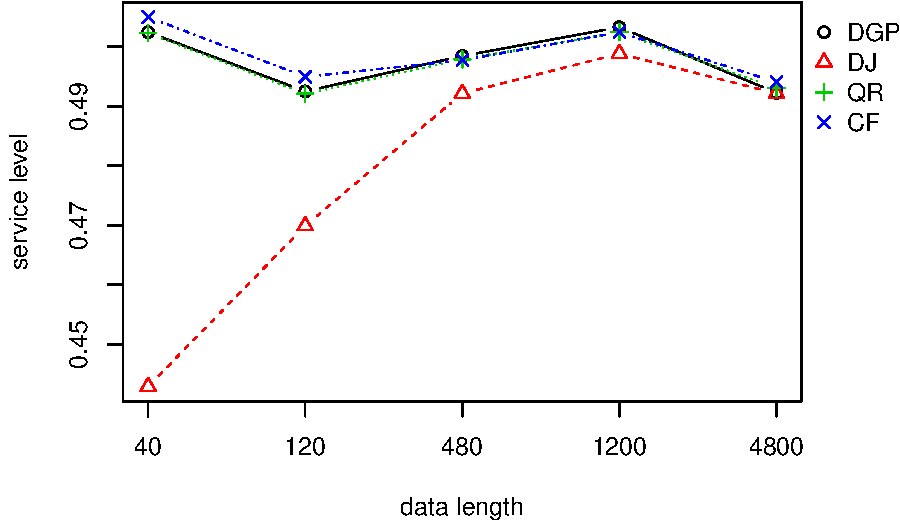
\includegraphics{linear-norm-plot_files/figure-latex/sl-1.pdf}
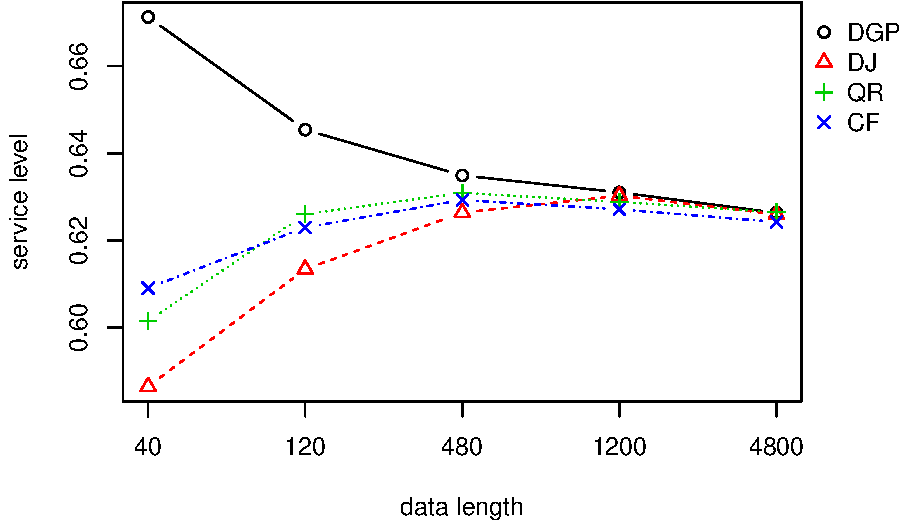
\includegraphics{linear-norm-plot_files/figure-latex/sl-2.pdf}
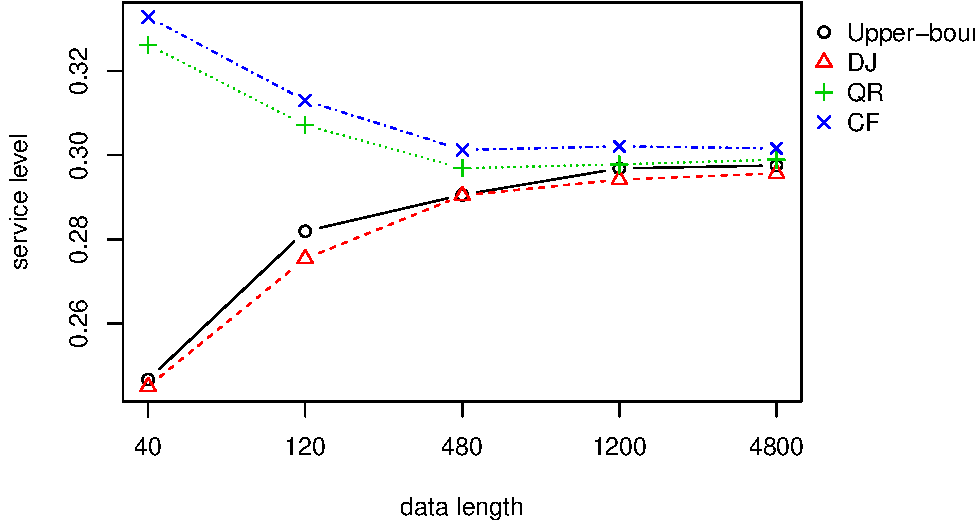
\includegraphics{linear-norm-plot_files/figure-latex/sl-3.pdf}

\begin{table}

\caption{\label{tab:Wilcoxon}p-value of Wilcoxon Test between data size 1200 and 4800}
\centering
\begin{tabular}[t]{ccccc}
\toprule
Target service level & DGP & disjoint & quantile & proposed\\
\midrule
\rowcolor{gray!6}  0.5 & 0.0244507 & 0.0090546 & 0.0784086 & 0.0393982\\
0.63 & 0.2033235 & 0.7949392 & 0.8106588 & 0.9501898\\
\rowcolor{gray!6}  0.3 & 0.2163362 & 0.0498548 & 0.8617589 & 0.4927552\\
\bottomrule
\end{tabular}
\end{table}

\begin{verbatim}
##            DGP        DJ        QR        CF
## 40   0.9739576 0.9587432 0.9694653 0.9704274
## 120  0.9744015 0.9679010 0.9728337 0.9731264
## 480  0.9742795 0.9707362 0.9737452 0.9738208
## 1200 0.9737634 0.9729700 0.9733849 0.9734056
## 4800 0.9745371 0.9742965 0.9742709 0.9742858
\end{verbatim}

\begin{verbatim}
##            DGP        DJ        QR        CF
## 40   0.9903111 0.9757714 0.9780703 0.9792021
## 120  0.9865163 0.9797998 0.9822862 0.9823411
## 480  0.9848323 0.9822811 0.9835870 0.9835376
## 1200 0.9847132 0.9839716 0.9841744 0.9841170
## 4800 0.9841651 0.9839729 0.9839263 0.9838614
\end{verbatim}

\begin{verbatim}
##            DGP        DJ        QR        CF
## 40   0.9259200 0.9212838 0.9481836 0.9514379
## 120  0.9439190 0.9395921 0.9515363 0.9527229
## 480  0.9506548 0.9465879 0.9523105 0.9526926
## 1200 0.9525118 0.9516110 0.9528853 0.9531534
## 4800 0.9532435 0.9529980 0.9528792 0.9530302
\end{verbatim}

\textbackslash begin\{table\}

\textbackslash caption\{\label{tab:size0.3}Size effect (q=30\%)\}
\centering \resizebox{\linewidth}{!}{
\begin{tabular}[t]{ccccccccccccc}
\toprule
\multicolumn{1}{c}{\textbf{ }} & \multicolumn{4}{c}{\textbf{Percentage profit loss}} & \multicolumn{4}{c}{\textbf{Service level}} & \multicolumn{4}{c}{\textbf{Fill rate}} \\
\cmidrule(l{3pt}r{3pt}){2-5} \cmidrule(l{3pt}r{3pt}){6-9} \cmidrule(l{3pt}r{3pt}){10-13}
Data size & DGP & disjoint & quantile & proposed & DGP & disjoint & quantile & proposed & DGP & disjoint & quantile & proposed\\
\midrule
40 & 2.7\% & 3.0\% & 2.9\% & 2.8\% & 0.15 & 0.18 & 0.33 & 0.34 & 92.6\% & 92.1\% & 94.8\% & 95.1\%\\
120 & 2.5\% & 2.7\% & 2.6\% & 2.6\% & 0.24 & 0.25 & 0.30 & 0.31 & 94.4\% & 94.0\% & 95.2\% & 95.3\%\\
480 & 2.5\% & 2.7\% & 2.5\% & 2.5\% & 0.29 & 0.29 & 0.31 & 0.31 & 95.1\% & 94.7\% & 95.2\% & 95.3\%\\
1200 & 2.4\% & 2.5\% & 2.5\% & 2.5\% & 0.29 & 0.29 & 0.30 & 0.30 & 95.3\% & 95.2\% & 95.3\% & 95.3\%\\
4800 & 2.5\% & 2.5\% & 2.5\% & 2.5\% & 0.30 & 0.30 & 0.30 & 0.30 & 95.3\% & 95.3\% & 95.3\% & 95.3\%\\
\bottomrule
\end{tabular}} \textbackslash end\{table\}

\begin{table}

\caption{\label{tab:level40}Target service level effect (n=40)}
\centering
\resizebox{\linewidth}{!}{
\begin{tabular}[t]{ccccccccc}
\toprule
\multicolumn{1}{c}{\textbf{ }} & \multicolumn{4}{c}{\textbf{Percentage profit loss}} & \multicolumn{4}{c}{\textbf{Service level}} \\
\cmidrule(l{3pt}r{3pt}){2-5} \cmidrule(l{3pt}r{3pt}){6-9}
Target service level & DGP & disjoint & quantile & proposed & DGP & disjoint & quantile & proposed\\
\midrule
\rowcolor{gray!6}  0.5 & 2.4\% & 2.7\% & 2.7\% & 2.7\% & 0.50 & 0.39 & 0.50 & 0.50\\
0.63 & 7.1\% & 7.6\% & 7.8\% & 7.5\% & 0.74 & 0.56 & 0.59 & 0.60\\
\rowcolor{gray!6}  0.3 & 2.7\% & 3.0\% & 2.9\% & 2.8\% & 0.15 & 0.18 & 0.33 & 0.34\\
\bottomrule
\end{tabular}}
\end{table}

\begin{table}

\caption{\label{tab:level480}Target service level effect (n=480)}
\centering
\resizebox{\linewidth}{!}{
\begin{tabular}[t]{ccccccccc}
\toprule
\multicolumn{1}{c}{\textbf{ }} & \multicolumn{4}{c}{\textbf{Percentage profit loss}} & \multicolumn{4}{c}{\textbf{Service level}} \\
\cmidrule(l{3pt}r{3pt}){2-5} \cmidrule(l{3pt}r{3pt}){6-9}
Target service level & DGP & disjoint & quantile & proposed & DGP & disjoint & quantile & proposed\\
\midrule
\rowcolor{gray!6}  0.5 & 2.3\% & 2.5\% & 2.4\% & 2.4\% & 0.50 & 0.49 & 0.50 & 0.50\\
0.63 & 6.6\% & 7.2\% & 6.8\% & 6.8\% & 0.65 & 0.63 & 0.64 & 0.63\\
\rowcolor{gray!6}  0.3 & 2.5\% & 2.7\% & 2.5\% & 2.5\% & 0.29 & 0.29 & 0.31 & 0.31\\
\bottomrule
\end{tabular}}
\end{table}

\begin{table}

\caption{\label{tab:level4800}Target service level effect (n=4800)}
\centering
\resizebox{\linewidth}{!}{
\begin{tabular}[t]{ccccccccc}
\toprule
\multicolumn{1}{c}{\textbf{ }} & \multicolumn{4}{c}{\textbf{Percentage profit loss}} & \multicolumn{4}{c}{\textbf{Service level}} \\
\cmidrule(l{3pt}r{3pt}){2-5} \cmidrule(l{3pt}r{3pt}){6-9}
Target service level & DGP & disjoint & quantile & proposed & DGP & disjoint & quantile & proposed\\
\midrule
\rowcolor{gray!6}  0.5 & 2.4\% & 2.4\% & 2.4\% & 2.4\% & 0.51 & 0.50 & 0.51 & 0.51\\
0.63 & 6.7\% & 6.7\% & 6.8\% & 6.8\% & 0.64 & 0.64 & 0.64 & 0.64\\
\rowcolor{gray!6}  0.3 & 2.5\% & 2.5\% & 2.5\% & 2.5\% & 0.30 & 0.30 & 0.30 & 0.30\\
\bottomrule
\end{tabular}}
\end{table}

\end{document}
